\section{evaluation results}
\label{sec:evaluationplan}
The approach is integrated into Papyrus Designer - an extension of Papyrus \cite{gerard201019}.
Papyrus Designer features component-based design in UML and full C++ code generation through embedding of fine-grained code as blocks of texts.
Formerly, it does not support model-code synchronization.
This section presents our evaluation results through experimentation. %with our model-code synchronization integrated into Papyrus Designer.

\begin {comment}
\subsection{Previous results}
%\vskip 0.1cm
\noindent
\tb{Semantic-conformance:}
We assess the preservation of UML semantics in the code.
In \cite{fullusm}, we show our experiments to test the runtime execution of the code against the precise semantics of UML State Machine standardized by OMG in \cite{PSSM} with a test suite consisting 66 test cases.
62 out of 66 cases passed leaving for future to fix the failed test cases.


%\vskip 0.1cm
\noindent
\tb{Standard code efficiency:}
We target resource-constrained embedded systems.
Hence, event processing speed and memory usage are critical.
We compare the efficiency of the generated code with the code generated by some UML tools and source code libraries in \cite{fullusm}.
The results show that the code in our approach runs fast and requires little memory.
\end{comment}

%\subsection{Synchronization evaluation through a case study}
%\vskip 0.1cm
%\noindent
%\tb{Synchronization correctness:}
The objective of experimentation is to evaluate the synchronization correctness of the synchronization of architecture model and code through a case study.
Three cases for the synchronization correctness are to be answered: (1) can the extended code be used to reconstruct the original architecture model? (2) if the extended code is modified, can the code modifications be propagated back to the model? and (3) if both extended code and model are concurrently modified, can our approach make the model and code consistent again?

\begin{comment}

RQ1: \ti{Right-invertibility - Can the extended code and mapping be used to reconstruct the original architecture model}? 

This question means to assess that not modifying the extended code (or
model, respectively) shall be reflected as not modifying the model
(respectively extended code). 
If no modifications are made to the code, the
model used for generating the code and the model received by
immediately reversing the generated code must be the same.

RQ1: \ti{Left-invertibility - If the extended code is modified, can the modifications made be propagated back to the model}?

In other words,  all modifications on the code
are captured and correctly propagated to the model by incremental reverse engineering so that the
modified code can be fully recreated by applying code generation
to the updated model.

RQ3: \ti{Concurrent modification - If both model and code concurrently modified, can our approach synchronize these two modified artifacts?}
\end{comment}


%We assess different cases
%Three cases are planned: (1) can the extended code and mapping be used to reconstruct the original architecture model? (2) if the extended code is modified, can the modifications made be propagated back to the model? and (3) if both extended code and model are concurrently modified, can the mapping be used for synchronization?

%\vskip 0.1cm
%\noindent
%\tb{Feasibility and scalability:}
We use our approach to develop an embedded software case study for LEGO. %, which is an embedded software for LEGO.
%Furthermore, if the approach can be applied to the case study and improve the development efficiency, we have shown its feasibility and it is likely that other development projects would also profit from it.
The LEGO car factory consists of small LEGO cars used for simulating a real industrial process \cite{lego}.
It is chosen for the evaluation because it is a real world embedded system with enough complexity.
%It is developed within our lab for demonstrating the Papyrus capabilities.
%It is previously developed by a developer using UML models and component-based engineering without a model-code synchronization mechanism. 

Previously, it was developed by using Papyrus Designer tool, which .   
%During the development, an architecture design model was created.
However, the developer felt difficult, unfamiliar, and annoyed to write fine-grained code within a limited textual editor supported by the tool.
The developer then refused to use that editor and programmed in CDT instead to be familiar and effective with programming facilities such as syntax highlights and auto-completion.
She then copied the code from CDT back to the model and regenerated the code.
The developer felt inefficient, prone-to-error, and lacked comprehension of the architecture information during code writing and copying. 
Furthermore, programming activities such as creation of methods are much easier in the code than in the model.
Because of these reasons, the LEGO car factory is suitable to the evaluation. 

A LEGO car is composed of four modules: chassis, front, back, and roof.% as in Fig. \ref{fig:legofactory}.
The communication between these modules is based on Bluetooth and master-slave like.
In the latter, the chassis acts as the master while the other modules as the slaves.
Each slave module consists of five components: bluetooth communication controller, convoyer, robotic arm, press, and shelf.	
The behavior of each component is described by a UML state machine.
The components communicate with each other through a data flow like communication schema.
Previously, each component holds references (pointers in C++), modeled as UML associations, to other components to exchange data between the components.
Furthermore, API invocations between these components were also aided by these references.
The latter, however, made the design not purely component-based and not reusable.

To adopt a fully component-based approach, we use flow ports to exchange data items/signals between the components within a module.
API invocations are re-designed by using service ports.   
Fig. \ref{fig:legofront} shows the UML composite structure diagram for the \ti{front} module without showing detailed structures of each of its components.
Furthermore, for simplification, only flow ports are shown in the figure.
The names of the signals/messages exchanged between flow ports of the components are annotated above connectors between the flow ports.
The three flow port types are used.
For example, the controller can send the \ti{StopProcess} signal to the other four components through its ports.
The robotic arm component can send/receive \ti{StopProcess} instances to the conveyor/from the controller through its bidirectional flow port respectively.  
Note that the processing of signals incoming to a component via its ports is realized by the component's state machine.

\begin{comment}
\begin{table}[]
	\centering
	\caption{Signal exchange between components}
	\label{my-label}
	\begin{tabular}{p{2.1cm}|p{1cm}|p{1cm}|p{1cm}|p{0.7cm}|p{0.7cm}}
		\backslashbox{Send}{Receive} & Controller & Conveyor & Robotic Arm & Shelf & Shelf \\ \hline \addlinespace
		Controller      &            &          &             &       &       \\ \hline
		Conveyor        &            &          &             &       &       \\ \hline
		Robotic Arm     &            &          &             &       &       \\ \hline
		Shelf           &            &          &             &       &       \\ \hline
		Press           &            &          &             &       &       \\
	\end{tabular}
\end{table}
\end{comment}

\subsubsection{Reconstruction of model from code}
In this first experimentation, for each (origin) module without fine-grained code embedded as blocks of text, we generated its corresponding extended code.
The model used for code generation contains 97 classes, 111 connectors, 119 ports, 15 state machines with 240 vertexes, 296 transitions and 11 events including signal and time events.
From the extended code, a reversed model was created by using the batch reverse engineering.
This reversed model was then compared with the origin module model.
No differences were detected for the four modules.
This result assesses that our approach and its implementation can be used for reconstructing a model from its corresponding generated code.
   
\subsubsection{Propagation of code modifications back to model}
In this second experimentation, for each of the extended code generated as above, we added class attributes and fine-grained code to each component.
Specifically, [how many?] state actions, transition effects, and class methods are created following the rules described in Section \ref{sec:mappingmechanism}.
Furthermore, API invocations between components through UML associations and C++ references are re-factored with the use of service ports and invocations through the required interface of a service port.

After enrichment for the generated code, we automatically propagated the code modifications back to the corresponding module model by using IRE.
We then manually checked the module model for updates as followings:

\begin{itemize}[\footnotesize]
	\item UML properties are created in the model corresponding to the class attributes in the code.
	
	\item UML state actions and transition effects are created within the model. Each has a block of text containing the fine-grained code filled in the extended code.
	
	\item UML operations are created in the model corresponding to the class methods in the code.
\end{itemize}

All of the model elements corresponding in the modified elements in the code were found in the updated model.
This result assesses that our approach and its implementation can propagate modifications in code back to model.

\begin{comment}
\begin{figure}
	\centering
	\includegraphics[clip, trim=0cm 9.7cm 15.0cm 0cm, width=\columnwidth]{figures/legofactory.pdf}
	\caption{LEGO factory modules} 
	\label{fig:legofactory}
\end{figure}
\end{comment}

\begin{figure}
	\centering
	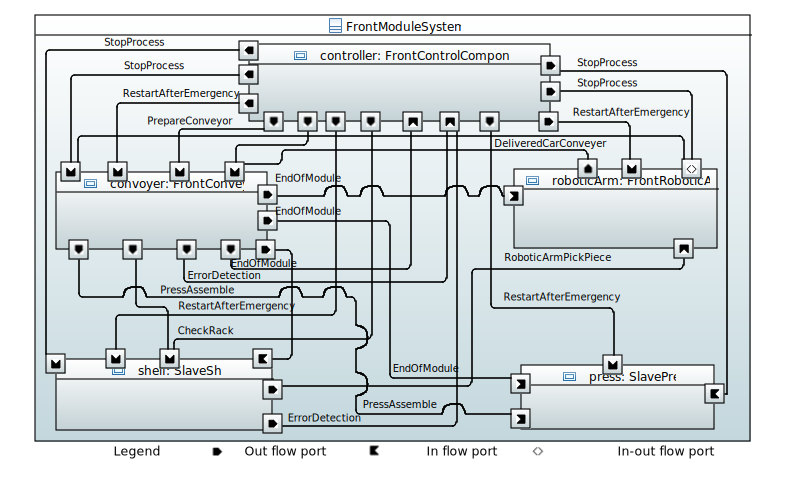
\includegraphics[clip, trim=1cm 0.5cm 1.2cm 0.2cm, width=\columnwidth]{figures/frontcomposite.pdf}
	\caption{Composite structure diagram of the front module for flow ports} 
	\label{fig:legofront}
\end{figure}


\subsubsection{Synchronization of concurrent modifications}
To assess our approach in case of concurrent modifications, we emulated a typical situation, in which the Lego architecture model, named the original model, and its generated code are concurrently modified.
To simplify the emulation, we only introduced modifications to method bodies in the code (become the \tb{modified code}) and additions of UML ports, connectors and states in the model (become the \tb{modified model}).

To synchronize the \tb{modified model} and \tb{modified code}, we used our previous synchronization mechanism \cite{foster2016}, whose steps are as followings:

\begin{itemize}[\footnotesize]
	\item Step 1: Through the IRE of the \tb{modified code}, the \tb{original model} is updated and becomes the \tb{code-updated original model}. 
	
	\item Step 2: Using EMF Compare to merge the model modifications from the \tb{modified model} to the \tb{code-updated original model}.
	The latter becomes the \tb{synchronized model}.
	
	\item Step 3: Re-generate to create the \tb{synchronized code} from the \tb{synchronized model} by using batch code generation.
\end{itemize}

To assess the consistency of the \tb{synchronized model} and \tb{synchronized code}, we use batch reverse engineering to create a \tb{reconstructed model}.
We then compare the \tb{reconstructed model} with the \tb{synchronized model}.
No differences were found during this comparison.
We assess that our approach can synchronize architecture model and code in case of concurrent modifications.



% Please add the following required packages to your document preamble:
% \usepackage{multirow}
\begin{table}[]
	\centering
	\caption{Lego Car Factory with and without synchronization}
	\label{table:compare}
	\begin{tabular}{|l|l|l|l|l|}
		\hline
		\multirow{2}{*}{Module} & \multicolumn{2}{l|}{Lines of code} & \multicolumn{2}{l|}{Binary size (KB)} \\ \cline{2-5} 
		& Without sync      & With sync      & Without sync   & With sync  \\ \hline
		Chassis                 & 9659               & \tb{11193}            & 256            & \tb{264}        \\ \hline
		Front                   & 9660               & \tb{12246}            & 248            & \tb{268}        \\ \hline
		Roof                    & 9725               & \tb{XX}            & 248            & \tb{XX}        \\ \hline
		Back                    & 9703               & \tb{XX}            & 248            & \tb{XX}        \\ \hline
	\end{tabular}
\end{table}

After the experimentations of the synchronization, we compared the generated code in our approach with the code generated from Papyrus Designer without the use of the synchronization.
Table \ref{table:compare} shows the comparison of the codes generated with and without our synchronization approach.
The number of lines of and the binary size compiled, by an ARM 32 bit Linux-based cross compiler, from code generated with our approach (With sync) are larger than those of the approach without synchronization.
However, the difference between the binary sizes of the executables is very subtle: our approach produces around 3\% larger (for the Chassis module), normalized to the binary size in case of the approach without synchronization.
This assesses that the proposed approach does not only bring the ability to synchronize UML-based architecture models and code, but also keeps the generated code quality acceptable.  


%The mapping and synchronization are feasible and scalable if efficient development is possible.

%Our research questions are as followings:
%\begin{description}[\footnotesize]
%	\item[\tb{RQ1}] A state machine \ttt{sm} is used for generating the front-end code. The latter is reversed engineered to produce another state machine \ttt{sm'}. Are \ttt{sm} and \ttt{sm'} identical? In other words: whether the front-end code generated from USMs model can be used for reconstructing the original model. This question is related to the \ti{GETPUT} law defined in \cite{foster_combinators_2007}.
	
%	\item[\tb{RQ2}] The back-end code is used for compilation. 
%	Does the runtime execution of the back-end code is semantic-conformant to Precise Semantics for UML State Machines (PSSM)? 
	
%	\item[\tb{RQ3}] Runtime performance and memory usage is undoubtedly critical in real-time and embedded systems. Particularly, in event-driven systems, the performance is measured by event processing speed. Does code generated by the presented approach outperform existing approaches and use less memory?
%\end{description} 

After the case study-based evaluation of our approach, we examines how scalable the approach is and our perspectives in the next section. 